% BEGIN TEMPLATE
\documentclass[11pt]{article}
\usepackage{graphicx}
\usepackage{hyperref} 
\usepackage{xcolor}
\usepackage{nameref}
\usepackage{listings}
\usepackage{float}
\usepackage[title]{appendix}
\usepackage[ruled]{algorithm2e}
\graphicspath{ {../../images/} }
\bibliographystyle{acm}
% CHANGE THESE
\newcommand{\courseListing}{CSCI 8360}
\newcommand{\courseName}{Machine Learning for Text}
\newcommand{\assignmentTitle}{Summary \#3}
\newcommand{\assignmentSubtitle}{Python K-Means}
\usepackage{geometry}
\geometry{margin=1in}

\hypersetup{
    colorlinks,
    linkcolor={red!50!black},
    citecolor={blue!50!black},
    urlcolor={blue!80!black}
}
\urlstyle{same}
\definecolor{codegreen}{rgb}{0,0.6,0}
\definecolor{codegray}{rgb}{0.5,0.5,0.5}
\definecolor{codepurple}{rgb}{0.58,0,0.82}
\lstdefinestyle{mystyle}{
    commentstyle=\color{codegreen},
    keywordstyle=\color{magenta},
    numberstyle=\tiny\color{codegray},
    stringstyle=\color{codepurple},
    basicstyle=\ttfamily\footnotesize,
    breakatwhitespace=false,         
    breaklines=true,                 
    captionpos=b,                    
    keepspaces=true,                 
    numbers=left,                    
    numbersep=5pt,                  
    showspaces=false,                
    showstringspaces=false,
    showtabs=false,                  
    tabsize=2
}

\lstset{style=mystyle}

\begin{document}
  \begin{center}
  
\includegraphics[scale=0.15]{UNO-Logo-Color.png}
  \\[0.3in]
  \textbf{\courseListing{}}\\
  \courseName{}
  \\[0.75in]
  \textbf{\assignmentTitle{}}\\
  \assignmentSubtitle{}
  \\[0.75in]
  \textbf{Patrick Davlin}
  \\[0.75in]
  \textbf{Computer Science Department}\\
  \textbf{Peter Kiewit Institute}\\
  \textbf{University of Nebraska}
  \\[0.75in]
  \textbf{Fall 2021}
  \\[0.3in]
  
\includegraphics[scale=0.075]{UNO-Icon-Color.png}
  \newpage
\end{center}
  \graphicspath{{./images/}}
\newpage
For this assignment, the primary task was to implement and observe the K-Nearest Neighbors (KNN) algorithm in Python.
In doing so, students were permitted to use any libraries necessary to implement the algorithm, with the intent being to observe the impact of various parameters on the algorithm.
With this in mind, a logical first step was to import the scikit-learn (\lstinline{sklearn}) package into the script and import its \lstinline{KNeighborsClassifier} subpackage.
Handily, \lstinline{sklearn} also has the 20 newsgroup dataset built in as well.

Like the prior assignment, with K-Means, the input data was vectorized prior to being fit into the model.
One difficulty encountered was that using separate training and testing data introduced differences in the shapes of data that were difficult to resolve with the vectorizer.
There's certainly some way to fix this, but to avoid overengineering a solution, it seemed easier to fetch all of the newsgroup data (training and testing) and then manually split it into training and testing groups.
After defining the classifier model, and specifying the number of neighbors $k$, the training group was used to fit the model by calling \lstinline{classifier.fit()}, and the predictions were obtained with \lstinline{classifier.predict()}.
Finally, the accuracy of the model was obtained with the \lstinline{accuracy_score()} function from \lstinline{sklearn} to assess how accurately the predictions were generated against the input labels.

To better understand the impact of changing the value of $k$, the model was run using $k$ values ranging from 1-20.
In addition, the nature of randomly splitting the data into training and testing groups meant that, functionally, there would be some variance in the training and testing groups. 
To reduce the impact of this, for each $k$-value the model was run ten times and the average accuracy was reported.
The model was also run with different test/train ratios, where the test data represented 60\% of the data, 40\% of the data, 20\% of the data, and 10\% of the data.
All said, the classification was evaluated six hundred times.
The results can be found in the \nameref{outputs} Appendix.

Speaking generally, classifying items into fewer groups was more effective.
This makes a lot of sense intuitively; the data set has a lot of overlap across technical and political categories, which was also reflected in the results from the K-Means experiment.
Therefore, making predictions with a smaller number of labels tended to be more accurate.
From $k=1$ to $k=9$, the accuracy score decreases linearly, and for $k > 10$, the results tend to stabilize for the smaller test sizes (e.g., the test runs where there was a higher ratio of training data to test data). In the largest test size, when $k > 10$, the results appear to become functionally random.
This is reflected with the declining values on the graph in the \nameref{outputs} Appendix.
That said, the results of the models were not particularly good--accuracy barely exceeded a score of 0.5 in exactly one case.
As expected, having fewer of the newsgroup items in the test groups led to more accurate results.
This is also fairly intuitive, since maximizing the amount of training time leads to better results in machine learning models.
Still, it was reassuring to know that the model could be improved with some small changes.

\newpage
\begin{appendices}
\section{KNN Visualization} \label{outputs}

\begin{figure}[H]
\centering
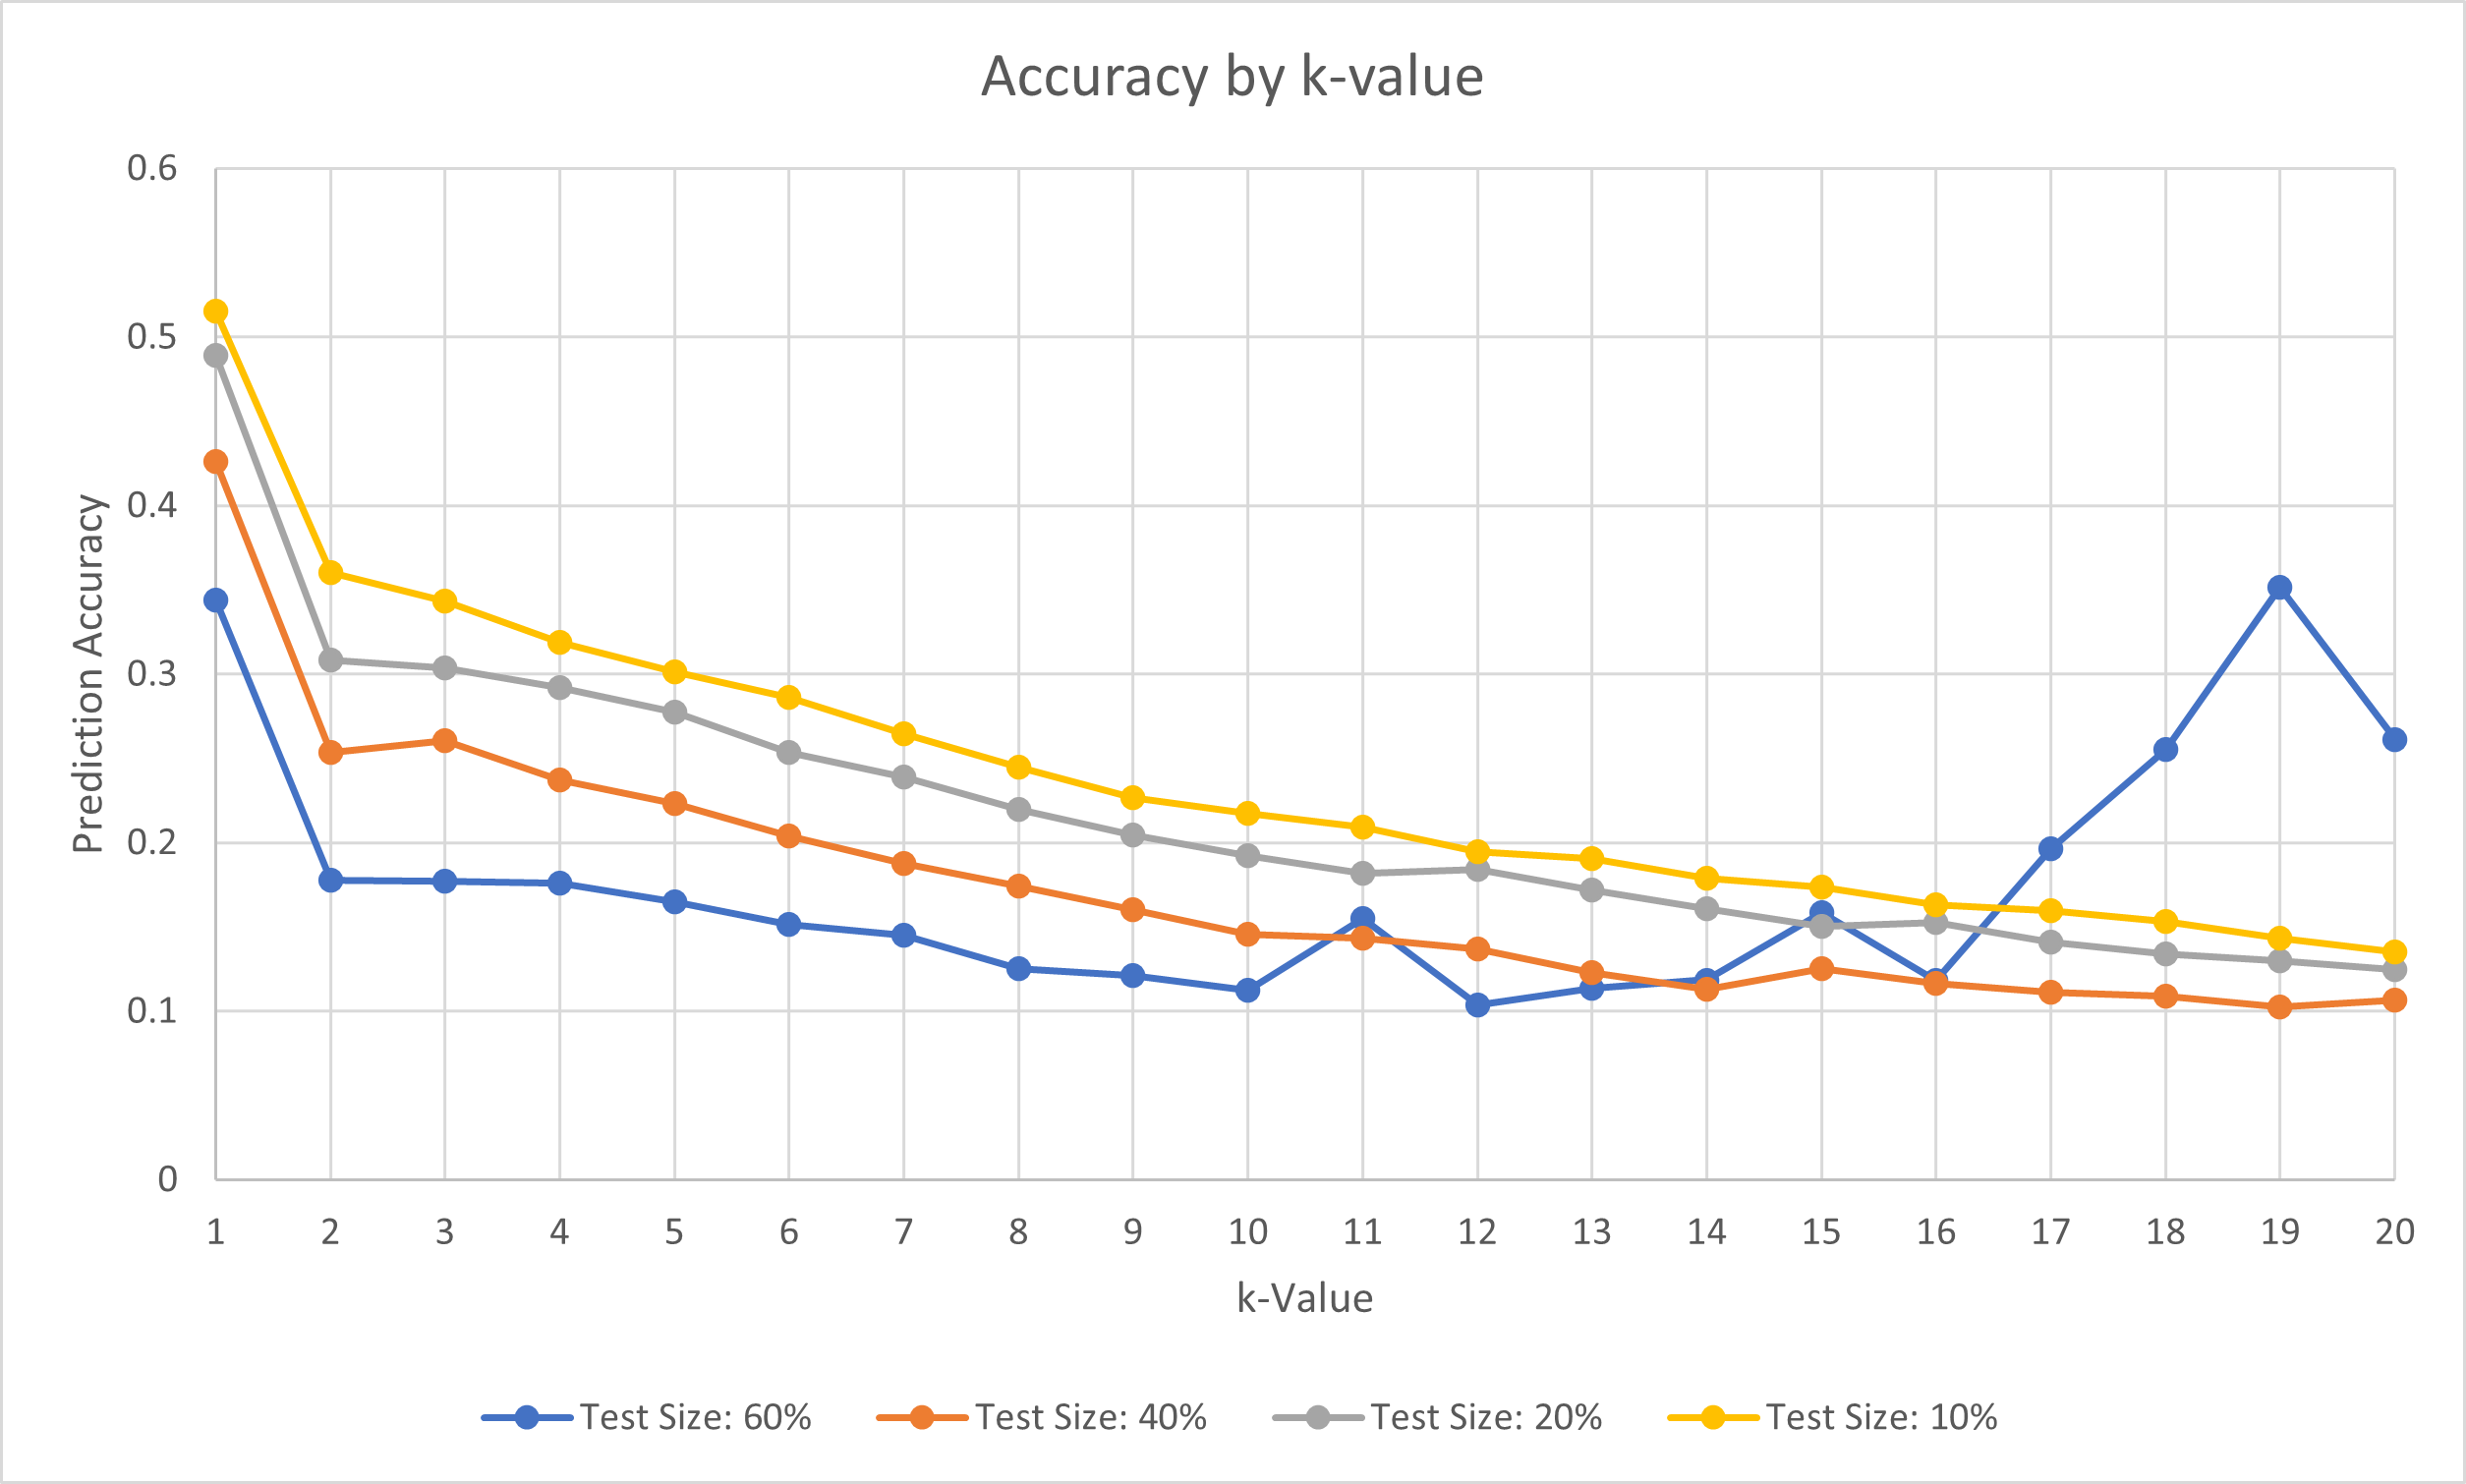
\includegraphics[width=6in]{images/knn.png}
\caption{Output from running}
\label{fig:out}
\end{figure}


\newpage
\section{Complete Code Listing} \label{codelist}
\lstinputlisting[language=Python]{knn.py}

\end{appendices}
  
\end{document}